%!TEX program = lualatex
\documentclass[a4paper,12pt]{article}
\usepackage{settings}
\usepackage{cancel}
\usepackage{ulem}
\newenvironment{task}{
    \par\noindent\textbf{Условие:}
}

\newenvironment{upd}
    {\par\noindent\textbf{Update:}}
    {\par\noindent\rule{\textwidth}{1pt}}

\newenvironment{solution}{
\begin{proof}[Решение]
    \mbox{}\par}
{\end{proof}}

\makeatletter
\newcommand\mathcircled[1]{%
  \mathpalette\@mathcircled{#1}%
}
\newcommand\@mathcircled[2]{%
  \tikz[baseline=(math.base)] \node[draw,circle,inner sep=1pt] (math) {$\m@th#1#2$};%
}
\makeatother

\setcounter{secnumdepth}{0}

\hypersetup{
    unicode=true,  % non-Latin characters in Acrobat’s bookmarks
    pdffitwindow=true,  % window fit to page when opened
    pdfstartview={FitH},  % fits the width of the page to the window
    pdfauthor={Котов А. А.},  % author
    pdfnewwindow=true,  % links in new PDF window
    colorlinks=true,  % false: boxed links; true: colored links
    linkcolor=linkcolor,  % color of internal links (change box color with linkbordercolor)
    citecolor=citecolor,  % color of links to bibliography
    filecolor=magenta,  % color of file links
    urlcolor=urlcolor  % color of external links
}

\definecolor{dkgreen}{rgb}{0,0.6,0}
\definecolor{gray}{rgb}{0.5,0.5,0.5}
\definecolor{mauve}{rgb}{0.58,0,0.82}  

\lstset{ %
language=python,                % the language of the code
basicstyle=\footnotesize,           % the size of the fonts that are used for the code
numbers=left,                   % where to put the line-numbers
numberstyle=\tiny\color{gray},  % the style that is used for the line-numbers
stepnumber=1,                   % the step between two line-numbers. If it's 1, each line 
                                % will be numbered
numbersep=5pt,                  % how far the line-numbers are from the code
backgroundcolor=\color{white},      % choose the background color. You must add \usepackage{color}
showspaces=false,               % show spaces adding particular underscores
showstringspaces=false,         % underline spaces within strings
showtabs=true,                 % show tabs within strings adding particular underscores
frame=single,                   % adds a frame around the code
rulecolor=\color{black!10},        % if not set, the frame-color may be changed on line-breaks within not-black text (e.g. comments (green here))
tabsize=4,                      % sets default tabsize to 2 spaces
captionpos=b,                   % sets the caption-position to bottom
breaklines=true,                % sets automatic line breaking
breakatwhitespace=false,        % sets if automatic breaks should only happen at whitespace
title=\lstname,                   % show the filename of files included with \lstinputlisting;
                                % also try caption instead of title
keywordstyle=\color{blue},          % keyword style
commentstyle=\color{dkgreen},       % comment style
stringstyle=\color{mauve},        % string literal style
escapeinside={\%*}{*)},            % if you want to add LaTeX within your code
morekeywords={done, to},              % if you want to add more keywords to the set
%  deletekeywords={...}              % if you want to delete keywords from the given language
}


\author{Котов Артем, МОиАД2020}
\title{Домашняя работа}
\date{\today}

\begin{document}
    \maketitle
    \tableofcontents
    \newpage
    
    Is it time to lakonichnyi solutions?
    --- Well\ldots it`s not
    %!TEX root = artem_kotov_v1.tex
\section{Task 1}

\begin{task}
    Вычисляем $p(a), p(b), p(c), p(d), p(c|a), p(c|b), p(c|d), p(c|ab), p(c|abd)$
\end{task}

\begin{solution}
    \begin{remark}
        $U[a,b] \sim \frac{1}{b - a + 1}[a \le x \le b]$
        $Bin(n, p) \sim {n \choose x} p^x (1 - p)^{n - x}$
    \end{remark}

    \begin{gather}
        p(a) = \frac{1}{16}[75 \le a \le 90] \\
        p(b) = \frac{1}{101}[500 \le b \le 600]
    \end{gather}
    Для вычисления $p(c)$ нам потребуется $p(c|ab)$ (для второй модели в целом, аналогично, разве что свертка упростится):
    \begin{gather}
        p_{\text{model}1}(c|ab) \sim \Bin(a, p_1) + \Bin(b, p_2) \sim \sum_i^c {a \choose i} p_1^i (1 - p_1)^{a - i} {b \choose c - i} p_2^{c - i} (1 - p_2)^{b - c + i} \\
        p_{\text{model}2}(c|ab) \sim \Poisson(ap_1 + bp_2)
    \end{gather}
    тогда
    \begin{equation}
        p(c) = \sum_{ab} p(c|ab)p(a)p(b) = \frac{1}{1616} \sum_{a = a_{\min}}^{a_{\max}} \sum_{b = b_{\min}}^{b_{\max}} \sum_{i = 0}^c {a \choose i} {b \choose c - i} p_1^i p_2^{c - i} (1 - p_1)^{a - i} (1 - p_2)^{b - c + i}.
    \end{equation}
    Но это не удобно программировать, лучше оставить в виде сверток двух биномиальных:
    \begin{equation}
        p(c|ab) = \sum_{x = 0}^c p(\Bin(a, p_1) = x) p(\Bin(b, p_2) = c - x)
    \end{equation}

    \begin{gather}
        p(c|a) = \sum_b p(c|ab)p(b) = \frac{1}{101} \sum_{b = 500}^{600} p(c|ab) \\
        p(c|b) = \sum_a p(c|ab)p(a) = \frac{1}{16} \sum_{a = 75}^{90} p(c|ab) \\
        p(c) = \sum_{ab} p(c|ab) \underbrace{p(a)p(b)}_{p(ab)}
    \end{gather}

    Теперь с $d$:
    \begin{gather}
        p(d|c) = p(c + \Bin(c, p_3) = d) = p(\Bin(c, p_3) = d - c) \\
        p(d) = \sum_c p(d|c)p(c) \\
        p(c|d) = \frac{p(d|c) p(c)}{p(d)} \\
        p(c|abd) = \frac{P(abcd)}{p(abd)} = \frac{p(d|c) p(c|ab) p(a) p(b)}{\sum_c p(d|c) p(c|ab) p(a) p(b)}
    \end{gather}
\end{solution}

    %!TEX root = kotov.tex
\section{Task 2}

\begin{task}
    Given $p(x) = \N(x|\mu, \Sigma)$ and $p(y|x) = \N(y|Ax, \Gamma)$, $p(x|y) = ?$
\end{task}

\begin{solution}
    \begin{gather}
        p(x|y) = \frac{1}{Z} p(y|x)p(x)
    \end{gather}

    Нормировочная константа $Z$ не содержит $x$, поэтому не будет нас сейчас интересовать в смысле вида распределения на $x$. Разберемся с числителем:
    \begin{gather}
        p(y|x)p(x) = \text{Const} \cdot \exp[-\frac12 ((x - \mu)^T \Sigma^{-1} (x - \mu) + (y - Ax)^T \Gamma^{-1} (y - Ax))]
    \end{gather}
    Разберемся с показателем экспоненты (опускаю $-\frac12$):
    \begin{gather}
        (x - \mu)^T \Sigma^{-1} (x - \mu) + (y - Ax)^T \Gamma^{-1} (y - Ax) \\
        = [\text{очередное раскрытие скобок}; \Sigma^T = \Sigma; \Gamma^T = \Gamma] = \\
        = x^T (\Sigma^{-1} + A^T \Gamma^{-1} A) x - 2(\mu^T \Sigma^{-1} + y^T \Gamma^{-1} A) x + C,
    \end{gather}
    т.е. с учетом $-\frac12$ получим экспоненту, у которой в показателе стоит отрицательно направленная парабола, после выделения полного квадрата которой получим, что это гауссово распределение с параметрами:
    \begin{gather}
        \mu' = (\Sigma^{-1} + A^T \Gamma^{-1} A)^{-1}(\Sigma^{-1} \mu + A^T \Gamma^{-1} y) \\
        \Sigma' = (\Sigma^{-1} + A^T \Gamma^{-1} A)^{-1},
    \end{gather}
    т.е.

    \begin{equation}
        p(x|y) = \N(x|(\Sigma^{-1} + A^T \Gamma^{-1} A)^{-1}(\Sigma^{-1} \mu + A^T \Gamma^{-1} y), (\Sigma^{-1} + A^T \Gamma^{-1} A)^{-1})
    \end{equation}

\end{solution}


    %!TEX root = kotov.tex
\section{Task 3}
\begin{task}
    Про поиск ближайших $k$ элементов к медиане
    \begin{enumerate}[(a)]
        \item по индексу
        \item по модулю разности значений
    \end{enumerate}
\end{task}

\begin{solution}
    \begin{enumerate}[(a)]
        \item
        За линейные времена найдем медиану $m$ и, например, $m-k/2$ статистику.
        \begin{remark}
            Где надо, там правильно округляем до целого.
        \end{remark}
        Затем, выкинем левую часть исходного массива, то есть ту часть, элементы в которой меньше, чем найденная статистика
        \begin{figure}[H]
            \centering
            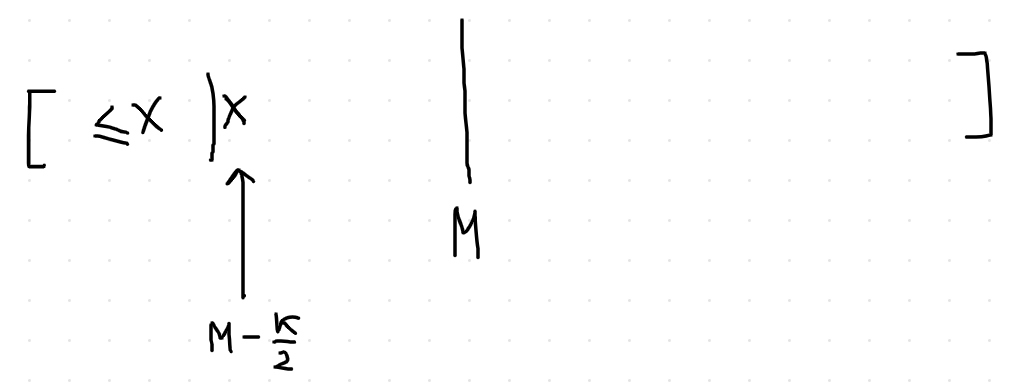
\includegraphics[scale=0.3]{pics/3_1.png}
            \caption{Художественная картинка, поясняющая слова}
        \end{figure}
        и будем рассматривать оставшуюся часть массива. Найдем в ней $k$-ую статистику (она соответствует $m+k/2$-ой статистике исходного массива). В ответ выводим элементы, от начала до найденной последней статистике.
        \item
        Сначала также найдем медиану $m$. Теперь создадим новый массив $b$, значения элементов которого $b_i = |a_i - m|$, где $a$ --- исходный массив. Эти все действия мы делали за $\O(n)$.
        
        Теперь в массиве $b$ найдем $k$-ую порядковую статистику (обозначим ее за $y$), тогда в массиве слева будет блок, элементы которого будут $< y$, берем в ответ начало этого массива до найденной $k$-ой порядковой статистики.
        \begin{remark}
            Имеется в виду, что мы запоминаем в пару индекс элементов из исходного массива, чтобы можно было потом легко восстановить значения самих элементов
        \end{remark}
        \begin{remark}
            Так как к этому моменту в массиве $b_i$ хранится ``расстояние'' элементов до медианы, то $k$-ая порядковая статистка в таком массиве говорит нам, какой элемент находится $k$-ым по счету по ``расстоянию'' до медианы.
        \end{remark}
    \end{enumerate}
\end{solution}
    %!TEX root = kotov.tex
\section{Task 4: Семейства функций}
\begin{solution}
    Важное предположение, я считаю в дальнейшем, что функции переводят каждый элемент их левого множества, в какие-то (необязательно различные, но единственные) элементы правого множества, вроде бы, это называется инъекцией.
    \begin{enumerate}
        \item Представим это себе как две доли графа, слева у нас $2^n$ вершин, справа --- $2^m$. Тогда нам комбинаторно надо посчитать кол-во различных ребер из левой доли в правую, т.е. по отношению каждой вершине справа задать вопрос, кто в нее приходит, тогда кол-во инъективных отображению $2^{m2^n}$.
        \item По определению, посчитаем вероятность, что $\forall x_1 \neq x_2: h(x_1) = h(x_2)$. Такая вероятность равна $P = \frac{\#\{h(x_1) = h(x_2)\}}{|H|} = 2^{m(2^n - 1)}/2^{m2^n} = \frac{1}{2^m} = \frac{1}{|\mathbb{F}_2^m|}$. То есть по определению для любых $n$ и $m$. Так же показывается и 2-независимость $\frac{\#\{h(x_1) = y_1, h(x_2) = y_2\}}{|H|} = \frac{2^{m(2^n - 2)}}{2^{m2^n}} = \frac{1}{(2^m)^2} = \frac{1}{|\mathbb{F}_2^m|^2}$
        \item Хм, стоит отметить, что бесконечности бывают разные, остановимся на случае счетного множества. Тогда, кажется, что сломается условие на произвольные $x$, но что-то не получается формально показать.
    \end{enumerate}
\end{solution}


\end{document}